\documentclass[a4paper]{article}

%% Language and font encodings
\usepackage[english,spanish]{babel}
\usepackage[utf8x]{inputenc}
\usepackage[T1]{fontenc}

\usepackage{hyperref}
\usepackage{caption}
\usepackage{subcaption}
\usepackage{booktabs}

%% Sets page size and margins
\usepackage[a4paper,top=3cm,bottom=2cm,left=3cm,right=3cm,marginparwidth=1.75cm]{geometry}

%% Useful packages
\usepackage{amsmath}
\usepackage{graphicx}
\usepackage[colorinlistoftodos]{todonotes}

\begin{document}

\title{%

\includegraphics[scale = 0.5]{./header_unc.png}\\[1.0 cm]	% University Logo
  Arquitectura de Computadoras \\
  \large Ingeniería en Computación FCEFyN - UNC\\
  		Trabajo Práctico 1 - ALU
  }


  \author{Izquierdo Agustina Mat: 37729473\\
          Salvatierra Andrés Mat: 39611008}
  
  \date{11 de septiembre de 2019}
\maketitle

\section{Introducción}

Para el primer trabajo práctico de la materia se realizó la implementación en FPGA de una Unidad Aritmética Lógica (ALU). Se desarrolló para la placa Basys 3 utilizando el software Vivado 2018.2. El módulo posee un bus de datos parametrizable. 

\begin{figure}[!htb]
\centering
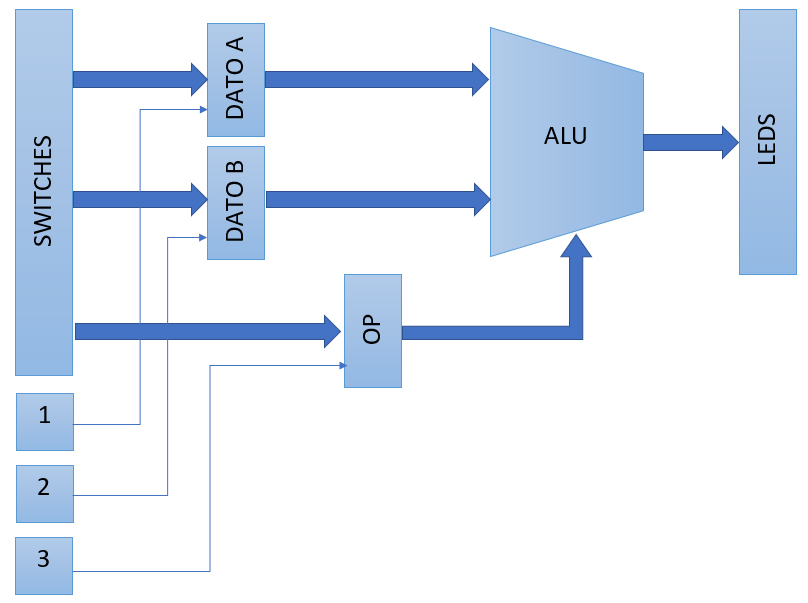
\includegraphics[width=.6\textwidth]{alu.jpg}
\caption{\label{fig:alu}Diagrama de la ALU}
\end{figure}

\newpage

La ALU soporta las siguientes operaciones, con los siguientes códigos:\\

\begin{table}[h]
\centering
\begin{tabular}{@{}ll@{}}
\toprule
Operación & Código \\ \midrule
ADD       & 100000 \\
SUB       & 100010 \\
AND       & 100100 \\
OR        & 100101 \\
XOR       & 100110 \\
NOR       & 100111 \\ 
SRA       & 000011 \\
SRL       & 000010 \\ \bottomrule
\end{tabular}
\caption{Operaciones de la ALU}
\label{operaciones}
\end{table}

\section{Desarrollo}

Para el desarrollo del módulo se definió un bloque llamado ALU, con los siguientes parámetros externos:
\begin{enumerate}
    \item NB\_DATA: numero de bits de los registros de entrada
    \item NB\_OPERADOR: numero de bits utilizado para representar las operaciones ya mencionadas
\end{enumerate}
Las siguientes entradas y salidas del modulo:
\begin{enumerate}
    \item i\_dato\_a [NB\_DATA -1 : 0]: entrada del modulo, dato a
    \item i\_dato\_b [NB\_DATA -1 : 0]: entrada del modulo, dato b
    \item i\_operador [NB\_OPERADOR -1 : 0]: entrada del modulo, representa la operación a realizar
    \item o\_resultado [NB\_DATA -1 : 0]: salida del modulo, representa el resultado de la operación
\end{enumerate}
Se desarrolló un módulo que se definió ALU\_toplevel, con los siguientes entradas y salidas:
\begin{enumerate}
    \item sw [NB\_DATA -1 : 0]: switches de entrada de datos por el bus
    \item btnL: botón izquierdo entrada dato a
    \item btnC: botón central entrada dato b
    \item btnR: botón derecho código de operación
    \item clk: entrada de clock
    \item led [NB\_DATA-1 : 0]: salida del resultado por los leds de la placa
\end{enumerate}
Para almacenar los valores ingresados se definieron dos registros A y B, que mantienen los números con los que se quiere operar. 
El resultado se almacena en el registro o\_resultado.\\

\section{Test Bench}

A la hora de realizar los tests del módulo se programó un test bench que compruebe el funcionamiento de cada una de las operaciones que debe realizar nuestra ALU, las simulaciones se realizaron con 5 bits.

\begin{enumerate}
\item Suma: 2 + 10 = 12
\item Suma con overflow: 10 + 10 = -12
\item Resta: 6 - 7 = -1
\item AND: 10101 \& 00111 = resultados
\item OR: 11001 | 01011 = 
\item XOR: 11111 \^ 01101 = no me dejo poner bien el operando aca
\item NOR: 00110 \~| 10001 = 
\item SRA: 10110 / 11 = no me dejo poner bien el operando aca
\item SRL: 10110 / 11 = no me dejo poner bien el operando aca
\end{enumerate}

El procedimiento fue codificar un clock simulado mediante una sentencia always, y dentro de un bloque initial escribir uno por uno los tests anteriores, simulando la entrada manual de los valores.

La siguiente captura de pantalla muestra los resultados de las anteriores pruebas de funcionamiento.

La primera fila representa el dato a, la segunda el dato b, la tercera la operación y la última el resultado obtenido.

% Capturas

\begin{figure}[!htb]
\centering
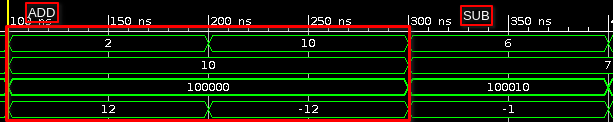
\includegraphics[width=1\textwidth]{Suma-Resta.png}
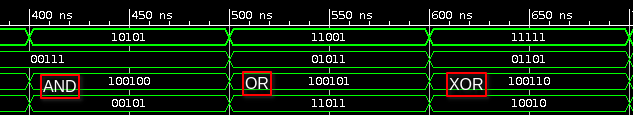
\includegraphics[width=1\textwidth]{AND-XOR.png}
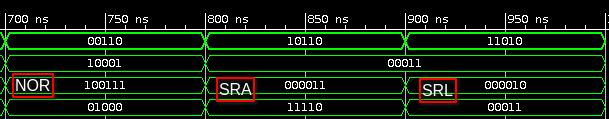
\includegraphics[width=1\textwidth]{NOR-SRL.jpg}
\caption{\label{fig:tests}Resultado del Test Bench}
\end{figure}

% 
\end{document}